\chapter{Installation and Exploitation --- quick-openstacked-hadoop}\label{cap:guiainstalacion}
\noindent To make a quick deployment in a single node and be able to run MapReduce workflows effortlessly, a \emph{git} repository has been set up with source files, configuration scripts, and the Hadoop VM. This guide will describe the steps required to achieve a basic installation.

\section{Quick Installation}\label{sec:instalacionqosh}

\subsection{System Requirements}\label{subsec:reqsis}
\noindent qosh's operating requirements:

\begin{itemize}
    \item x86\_64 CPU with virtualization extensions (VT-x or AMD-V).
    \item 4 GB of RAM or more.
    \item 10 GB of HDD space.
    \item Fedora 17 installation.
\end{itemize}

The amount of RAM and HDD will limit the number of concurrent instances that are allowed to run --- recall that each instance will be provisioned 1 GB of RAM and 4 GB of HDD on boot from the host computer.

\subsection{Installation}\label{subsec:instalacion}
\noindent Figure \ref{fig:comandosshel} contains the command list that will have to be typed in a terminal to run the installation and configuration scripts.

\begin{figure}[tbp]
 \begin{center}
  \begin{tabular}{|l|}
   \hline
   \texttt{{\bf \$} sudo yum install -y git} \\
   \texttt{{\bf \$} sudo yum update -y} \\
   \texttt{{\bf \$} sudo reboot} \\ \\
   \texttt{{\bf \$} cd <destination\_folder>} \\
   \texttt{{\bf \$} git clone https://code.google.com/p/quick-openstacked-hadoop} \\
   (quick-openstacked-hadoop folder will be created) \\ \\
   \texttt{{\bf \$} cd quick-openstacked-hadoop} \\
   \texttt{{\bf \$} sudo python install.py} \\
   (OpenStack Folsom, Hadoop VM, Fabric and Django will be installed) \\ \\
   \texttt{{\bf \$} python configure.py} \\
   (Django will be adjusted) \\
   \hline
  \end{tabular}
  \caption{Command sequence I}
  \label{fig:comandosshell}
 \end{center}
\end{figure}

\subsection{Test-driving the Setup}\label{subsec:testejecucion}
\noindent If the commands in the previous section have succeeded, OpenStack and Django should be correctly installed. To assert this, open \url{http://localhost/dashboard} in a web browser. After a few seconds there should appear the welcoming Horizon splash screen that would allow to log into OpenStack --- user name and password default to \emph{udc}. Once logged in, a web page like the one in figure \ref{fig:homeos} should be displayed.

\begin{figure}[tbp]
\begin{center}
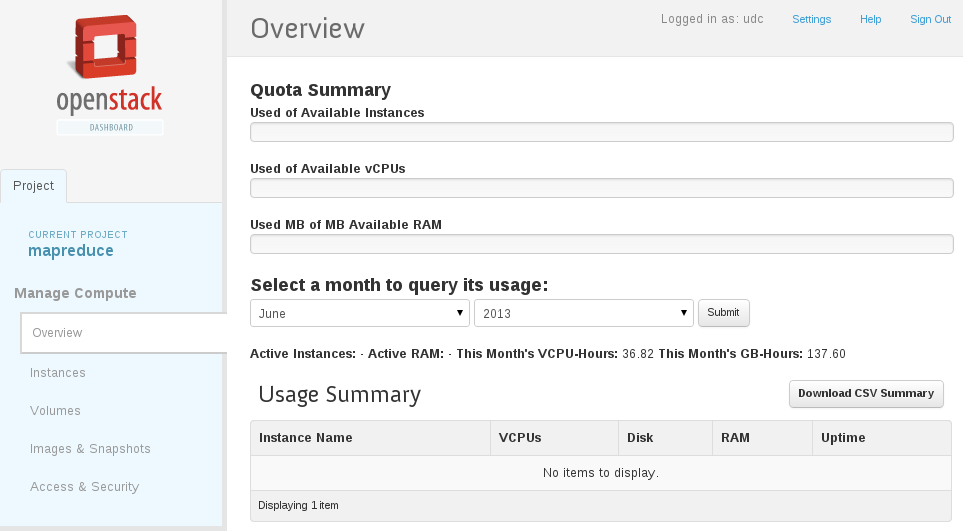
\includegraphics[width=0.99\textwidth]{imagenes/045.png}
\caption{OpenStack Folsom overview page}
\label{fig:homeos}
\end{center}
\end{figure}

At this point Django's development web server may be started to directly interact with qosh and check whether its installation succeeded --- figure \ref{fig:comandlsshell2} shows the command sequence to start the server. Again, a web browser shall be used to open \url{http://localhost:8000/albaproject/mapred}; then, qosh log in interface should load. Username and password are \emph{udc} again --- recall that user access is delegated entirely to OpenStack Keystone. Figure \ref{fig:comandosshell2} lists the commands that should be typed in a terminal.

\begin{figure}[tbp]
    \begin{center}
        \begin{tabular}{|l|}
            \hline
            \texttt{{\bf \$} cd quick-openstacked-hadoop/Alba/albaproject} \\
            \texttt{{\bf \$} python manage.py runserver} \\
            \hline
        \end{tabular}
        \caption{Command sequence II}
        \label{fig:comandosshell2}
    \end{center}
\end{figure}

\subsection{Testing a Workflow for Hadoop}\label{subsec:flujohadoop}
\noindent Finally, to ensure every component is completely installed and configured, a real MapReduce workflow should be run in qosh. Input files for this test case might be downloaded from \url{https://code.google.com/p/quick-openstacked-hadoop/downloads/list} (\texttt{just\_imagine.tar.gz} and \texttt{bigtxt.tar.gz} --- zipped files containing plain-text files whose words will be counted --- and \texttt{wordcount.jar} --- package containing the classical word count MapReduce implementation.

Just after logging in, qosh's main page should load on screen. From there, \emph{Define Job} shall be clicked and the form that sets up the MapReduce job should appear. The fields should be filled in in a similar way as in figure \ref{fig:defmapredjob} before clicking \emph{launch} to begin the process. Once the job be completed the results may be downloaded from the \emph{Job History} page.

\begin{figure}[bp]
\begin{center}
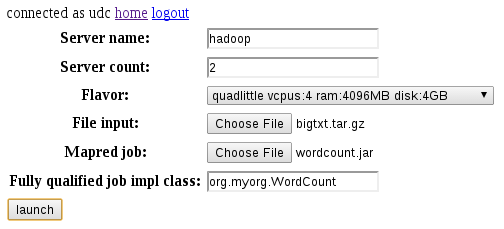
\includegraphics[width=0.90\textwidth]{imagenes/046.png}
\caption{MapReduce job definition}
\label{fig:defmapredjob}
\end{center}
\end{figure}

The image \ref{fig:mapredjobhistory} captures the \emph{Job History} page, and the image \ref{fig:mapredjobdetails} shows a capture detailing job \#56 from the \ref{Job Details} page.

\begin{figure}[tbp]
\begin{center}
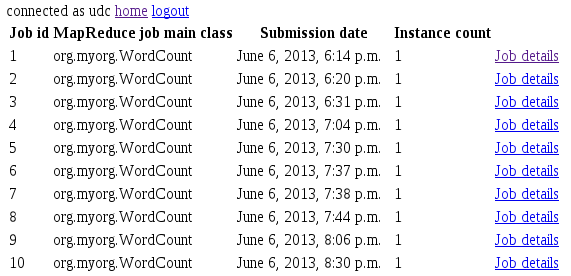
\includegraphics[width=0.99\textwidth]{imagenes/047.png}
\caption{MapReduce Job History}
\label{fig:mapredjobhistory}
\end{center}
\end{figure}

\begin{figure}[tbp]
\begin{center}
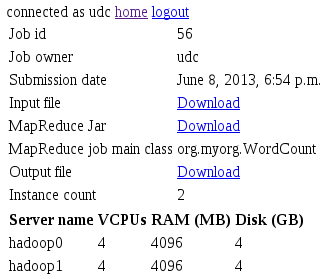
\includegraphics[width=0.60\textwidth]{imagenes/048.png}
\caption{Job \#56 details}
\label{fig:mapredjobdetails}
\end{center}
\end{figure}

\section{Long-term Operation}\label{sec:explotacionqosh}
\noindent To send MapReduce workflows into qosh, the operating procedure described in section \ref{subsec:flujohadoop} should be followed. Changing job options, cluster size, and main class may be accomplished by filling the form fields according to the user's needs.

By default qosh is configured to run in debug mode. This behavior may be easily modified by altering the flag \textbf{DEBUG} within \texttt{settings.py}. Furthermore, it should be noted that qosh will operate much faster when deployed to a production-level web server.

OpenStack Compute will keep a log in \texttt{/var/log/nova} that could be read should any issue appeared. By default, workflow computed results will be stored to \texttt{\$HOME/Public} which may be changed in \texttt{settings.py}, variable \textbf{MEDIA\_ROOT}.
